\section{Literature Review}
\paragraph{}In a (Proton Electron Membrane)PEM fuel cell stack, chemical energy from the reaction between hydrogen and oxygen is converted directly into electric energy. Water and heat are produced as by-products.
\begin{figure}[!h]
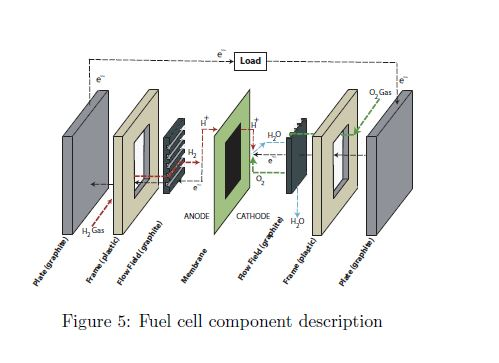
\includegraphics{Figures/Figure4}
\caption{Fuel cell component description
\cite{stefanopoulou_mechatronics_nodate}}
\end{figure} 
\paragraph{}In the figure above, hydrogen travels through inlet manifolds to the flow fields. From the flow fields, gas diffuses through porous media to the membrane. The membrane, which is sandwiched in the middle of the cell, contains catalyst and microporous diffusion layers along with gaskets as a single integrated unit. One side of the membrane is  the anode and the other is the cathode. The anode and cathode are more generally referred to as electrodes. The catalyst layer at the anode separates hydrogen molecules into protons and electrons
